\documentclass[7pt]{beamer}
\usepackage{beamerthemesplit}
\usepackage{amsfonts}
\usepackage{amsmath}		
\usepackage{amssymb}
\usepackage{float}
\usepackage{graphicx}
\usepackage{longtable}
\usepackage{makeidx}
\usepackage{rotating}
\usepackage{wasysym}

%\usepackage[latin2]{inputenc}
%\usepackage[romanian,magyar]{babel}
\usepackage{graphicx}
%\usepackage{dsfont}
\usepackage{beamerthemesplit}
\usepackage{hyperref}
\usepackage{caption}
\definecolor{red}{RGB}{0,0,200}
\mode<presentation>
{
\newtheorem{dfn}{Definition}[section]
\newtheorem{lem}[dfn]{Lemma}
\newtheorem{thm}[dfn]{Theorem}
\newtheorem{prop}[dfn]{Proposition}
\newtheorem{rem}[dfn]{Remark}
\newtheorem{cor}[dfn]{Corollary}
\newtheorem{ex}[dfn]{Example}
\newtheorem{pf}[dfn]{Proof}
%\newtheorem{notn}[dfn]{Notation.}
\newcommand{\R}{\mathbb R}
\newcommand{\F}{\mathbb F}
\newcommand{\C}{\mathbb C}
\newcommand{\N}{\mathbb N}
\newcommand{\Z}{\mathbb Z}
\newcommand{\Q}{\mathbb Q}
\newenvironment{notn}[1][Notation]{\noindent\textbf{#1.} }{\ \rule{0.0em}{0.0em}}
%Defining Caligraphic letters
\newcommand{\calL}{\mathcal{L}}
\newcommand{\calN}{\mathcal{N}}
\newcommand{\calP}{\mathcal{P}}
\newcommand{\calB}{\mathcal{B}}
\newcommand{\calO}{\mathcal{O}}
\newcommand{\calK}{\mathcal{K}}
\newcommand{\calG}{\mathcal{G}}
\newcommand{\calD}{\mathcal{D}}
\newcommand{\calU}{\mathcal{U}}
\newcommand{\calR}{\mathcal{R}}
%\begin{comment}
\newcommand{\al}{\alpha}
\newcommand{\be}{\beta}
\newcommand{\ga}{\gamma}
\newcommand{\Ga}{\Gamma}
\newcommand{\te}{\theta}
\newcommand{\et}{\eta}
\newcommand{\om}{\omega}
\newcommand{\Om}{\Omega}
\newcommand{\ps}{\psi}
\newcommand{\Ps}{\Psi}
\newcommand{\daba}{\partial}
%\newcommand{\p}{\pi}
\newcommand{\ph}{\phi}
\newcommand{\de}{\delta}
\newcommand{\ro}{\rho}
\newcommand{\si}{\sigma}
\newcommand{\Si}{\Sigma}
\newcommand{\la}{\lambda}
%\newcommand{\m}{\mu\psi}
\newcommand{\vp}{\varphi}
\newcommand{\ep}{\varepsilon}
\newcommand{\id}{\,\mathrm{d}}




%\setbeamertemplate{itemize item}[ball]

  \useoutertheme{infolines}
  \usetheme[hideothersubsections]{Berkeley}
  \usecolortheme[named=red]{structure}
  \usecolortheme{whale}
  \useinnertheme{rounded}
  \usefonttheme[onlymath]{serif}
  \setbeamertemplate{blocks}[rounded][shadow=true]
  \setbeamertemplate{navigation symbols}{}
  \usecolortheme{sidebartab}
}
%====================================================================================
% SLIDE 1: TITLE
%====================================================================================

\title[Bathymetry Inversion from Waves]{Inverting for Near Coastal Bathymetry from Surface Wave Properties}
\author[]{ 
Lasith Adhikari, Charnelle Bland, \\
Lopamudra (Monty) Chakravarty, Wenbin Dong, \\
Olaniyi Samuel Iyiola, Gail Muldoon, Clint Seinen \\
\vspace{5mm}
Supervised by\\ Ty  Hesser (USACE) \& Lea Jenkins (Clemson)
}
\institute[IMSM]{Industrial Mathematical and Statistical Modeling Workshop}
\date{July 2016}
%\logo{\includegraphics[height=1.4cm,width=1.5cm]{aust_logo}}
\begin{document}
\frame{\titlepage}

%======================================================================================
%======================================================================================
\section{Introduction}
%======================================================================================
%======================================================================================

%======================================================================================
%SLIDE 2
%======================================================================================
\begin{frame}
    \frametitle{Many coastal processes are affected by bathymetry}
        \begin{columns}
            \column{0.5\textwidth}           
                \begin{figure}[h!]
                		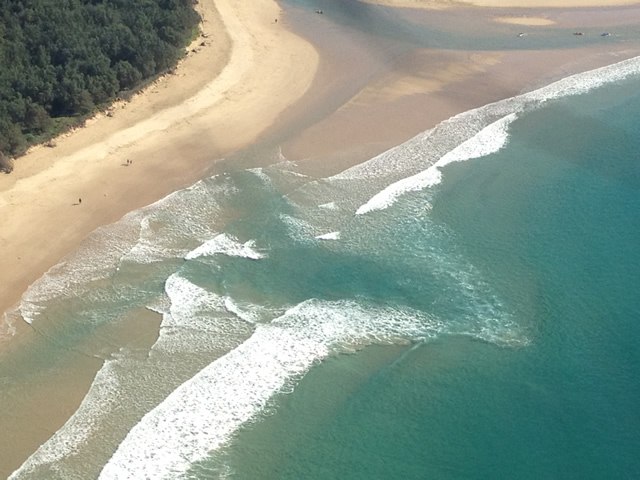
\includegraphics[width=1\linewidth]{img/Rip_C.jpg}\hfill
                \end{figure}              
            \column{0.5\textwidth}
                \begin{figure}
                		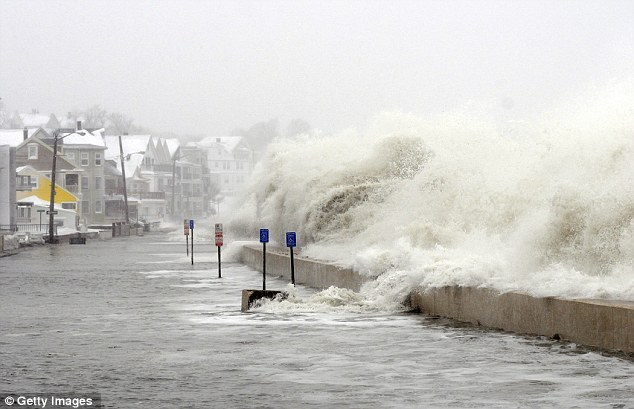
\includegraphics[width=1\linewidth]{img/C_Flood.jpg}\vfill
               		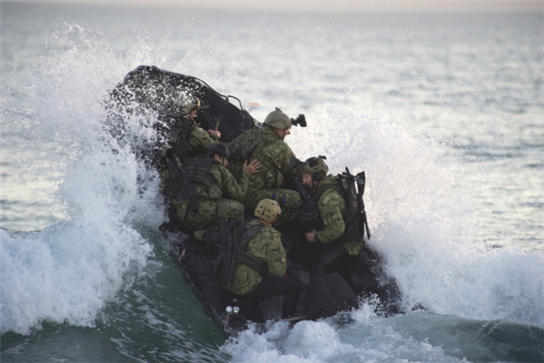
\includegraphics[width=1\linewidth]{img/Navy_S.jpg}
                \end{figure}       
        \end{columns}
\end{frame}


%======================================================================================
% SLIDE 3
%======================================================================================
\begin{frame}
	\frametitle{Bathymetry is submarine topography}
		\begin{figure}[h]
			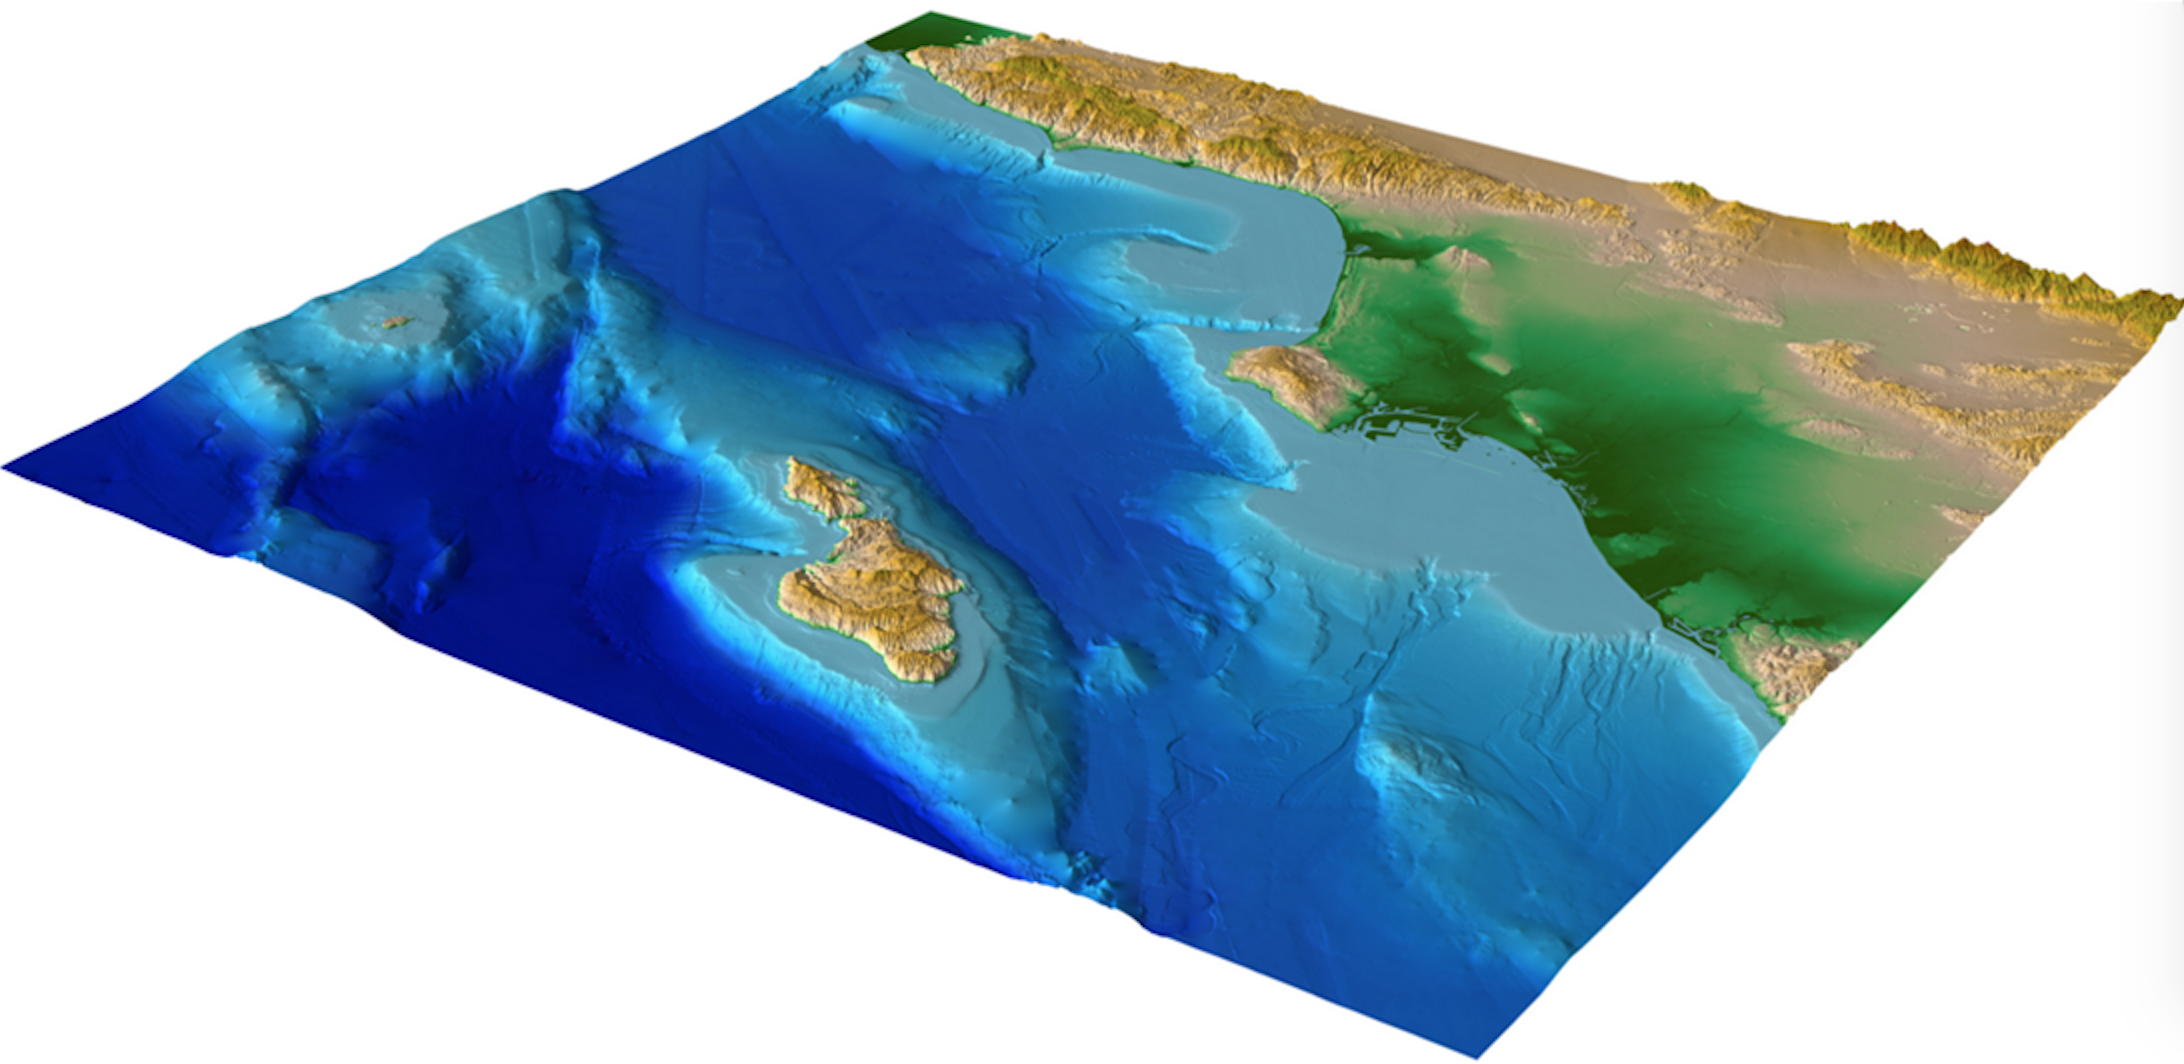
\includegraphics[width=1.\linewidth]{img/bath_topo_example.png}\hfill
		\end{figure}
\end{frame}

%=====================================================================================
% SLIDE 4
%======================================================================================
\begin{frame}
    \frametitle{Direct measurements are expensive and challenging}

    \begin{columns}
    
        \column{0.5\textwidth}
            \centering
            \begin{figure}[h!]
                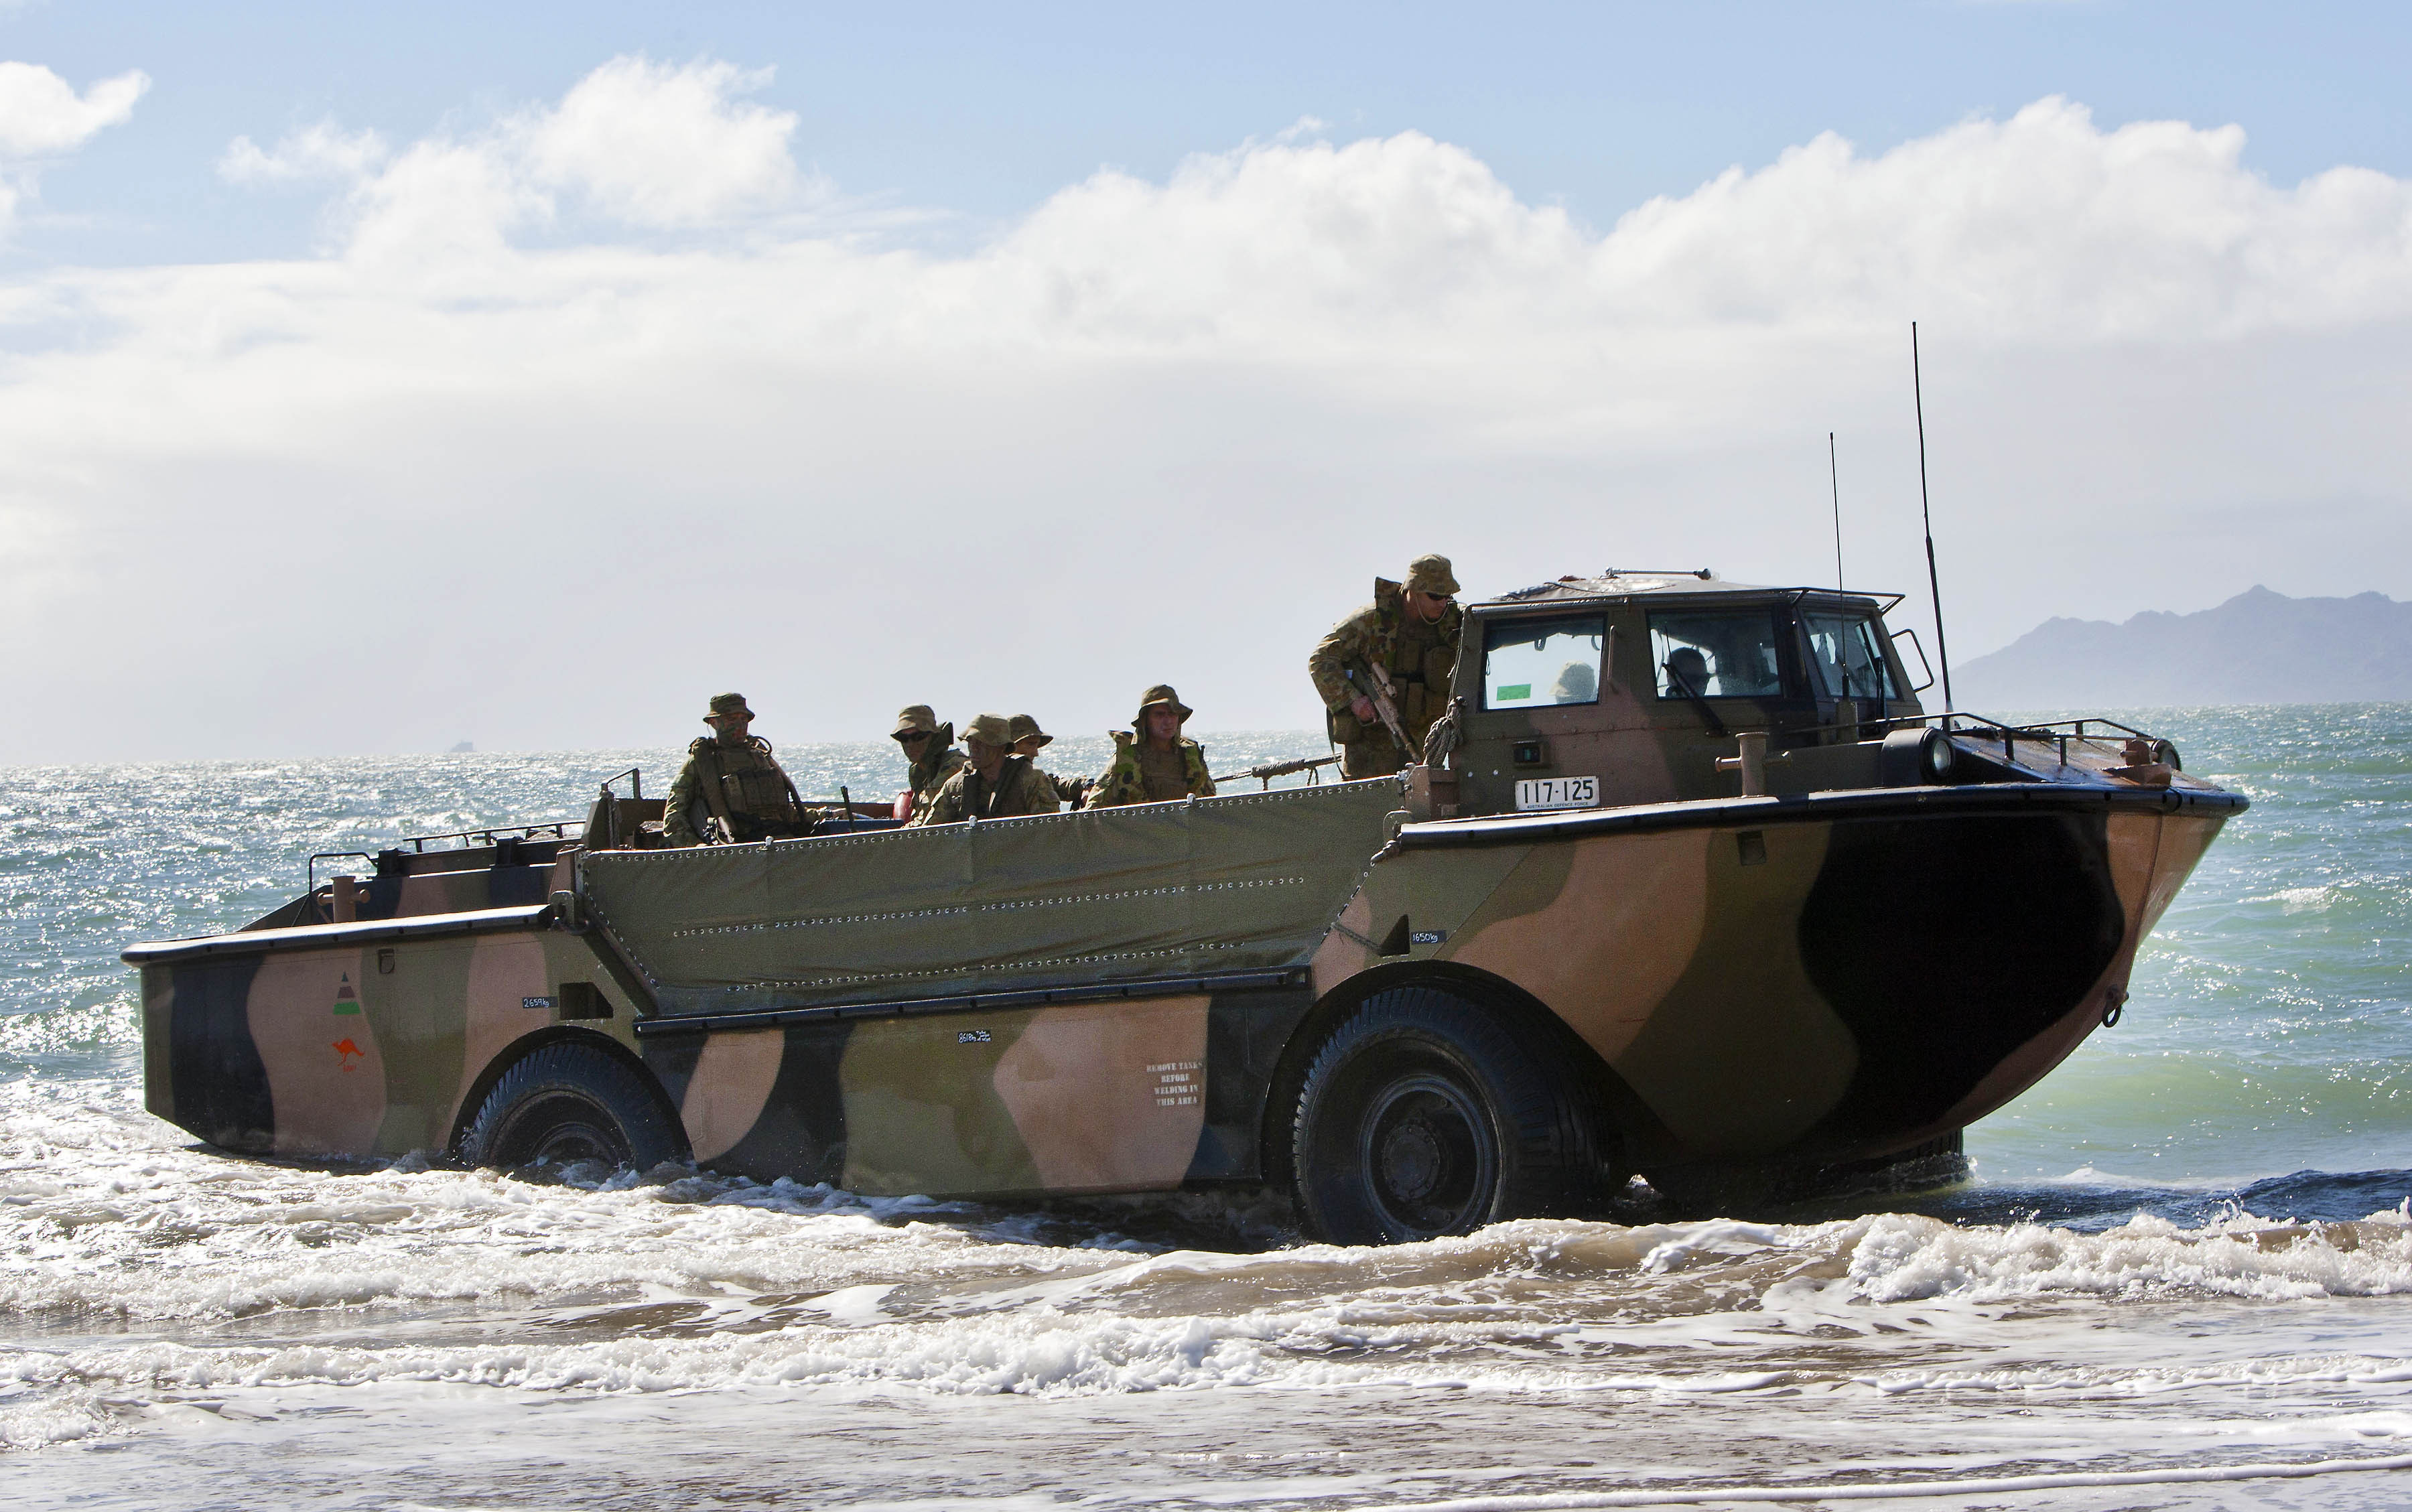
\includegraphics[width=1\linewidth]{img/LARC2.jpg}\hfill
                \centering
                \captionsetup{labelformat=empty}
                \caption{LARC}
            \end{figure}
        
        \column{0.5\textwidth}
            \begin{figure}[h]
                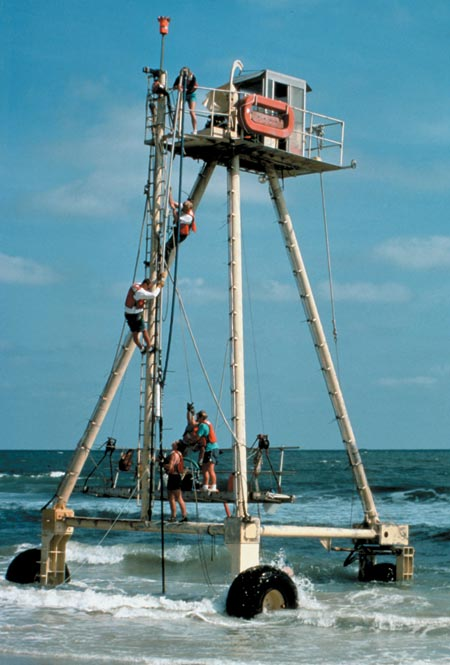
\includegraphics[width=0.8\linewidth]{img/CRAB3.JPG}
                \captionsetup{labelformat=empty}
                \caption{CRAB}
            \end{figure}
    
    \end{columns}
\end{frame}

%=====================================================================================
% SLIDE 5
%=====================================================================================
\begin{frame}
    \frametitle{Inverse models estimate depth using data \& physics}
    
    	\begin{figure}[H]
	 	\centering
	 	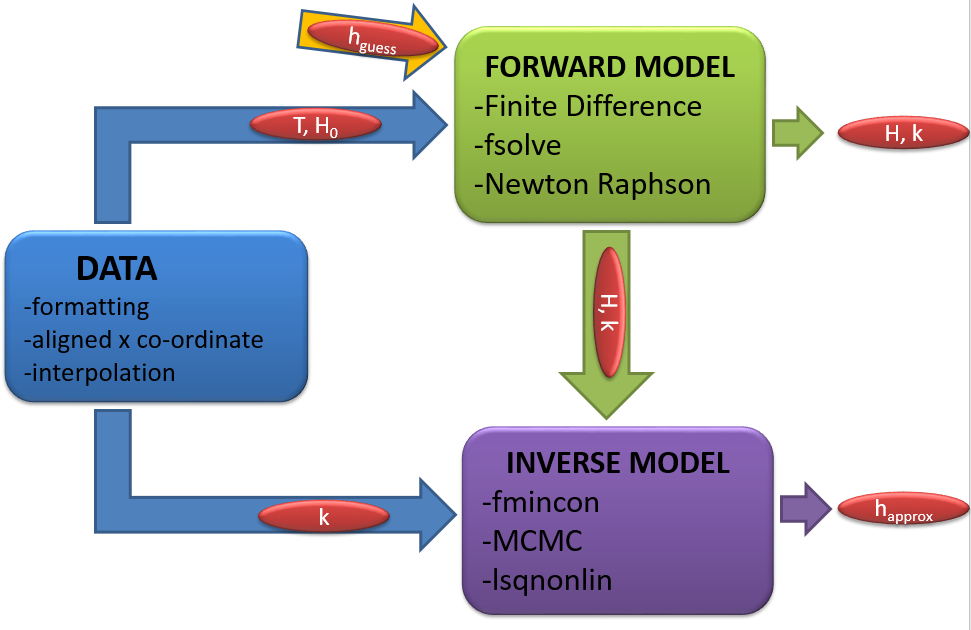
\includegraphics[width=1.0\linewidth]{img/Flow_C.png}
	\end{figure}
\end{frame}

%=====================================================================================
%SLIDE  6
%=====================================================================================
\begin{frame}
    \frametitle{Bathymetry is related to surface wave properties}
        \begin{figure}[flowchart]
            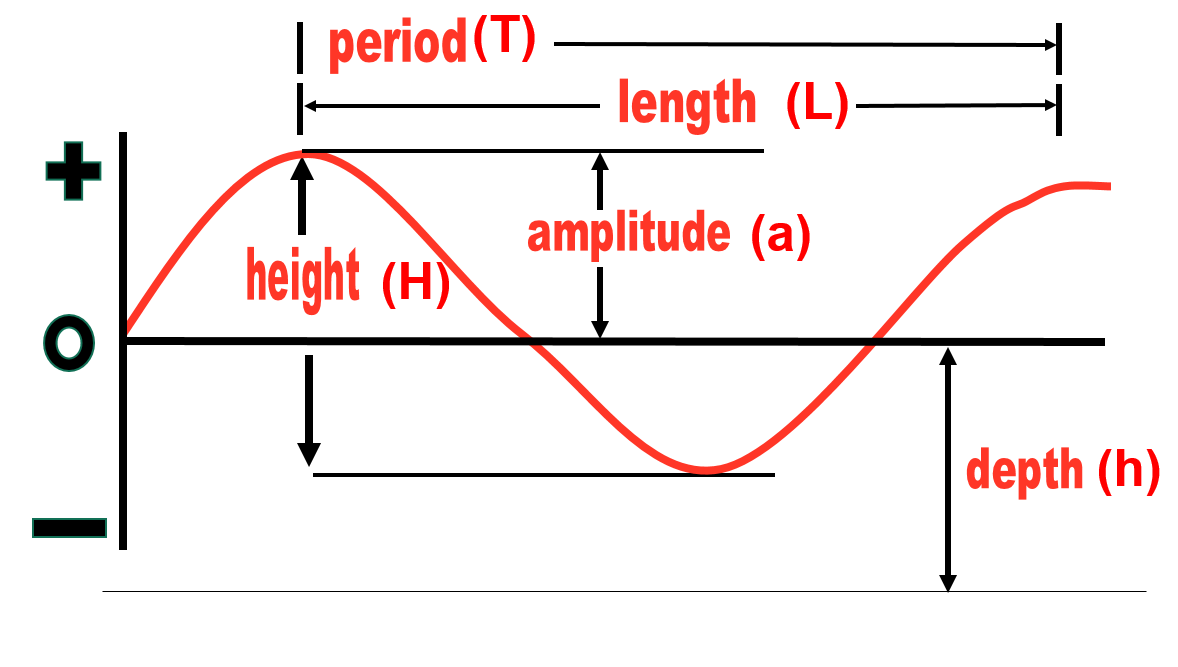
\includegraphics[width=1.0\linewidth]{img/Wave.jpg}
        \end{figure}
        \centering
        \begin{equation}
        		k = \frac{2\pi}{L}
        \end{equation}
\end{frame}



%====================================================================================
%====================================================================================
\section{Data}
%====================================================================================
%====================================================================================

%====================================================================================
% SLIDE  7
%====================================================================================
\begin{frame}
    \frametitle{Before we invert we need data}
        \begin{figure}[flowchart]
        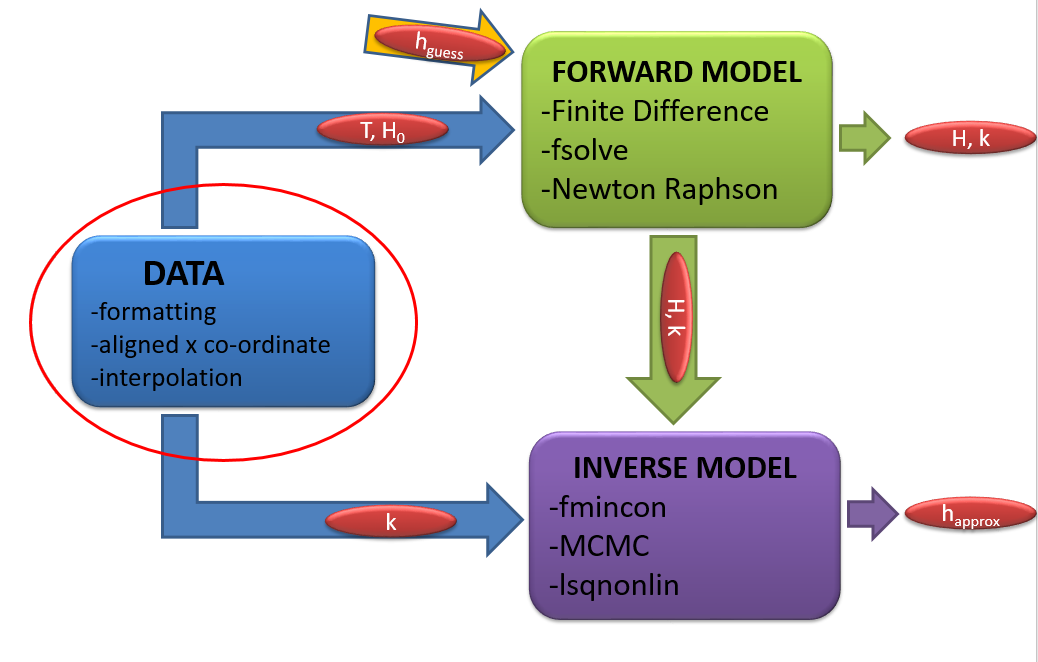
\includegraphics[width=1.0\linewidth]{img/Focus_D.png}
        \end{figure}
\end{frame}

%====================================================================================
%SLIDE   8
%====================================================================================
\begin{frame}
	\frametitle{Data was collected by the  USACE in Duck, NC}
		 \centering
		 \begin{figure}
       			 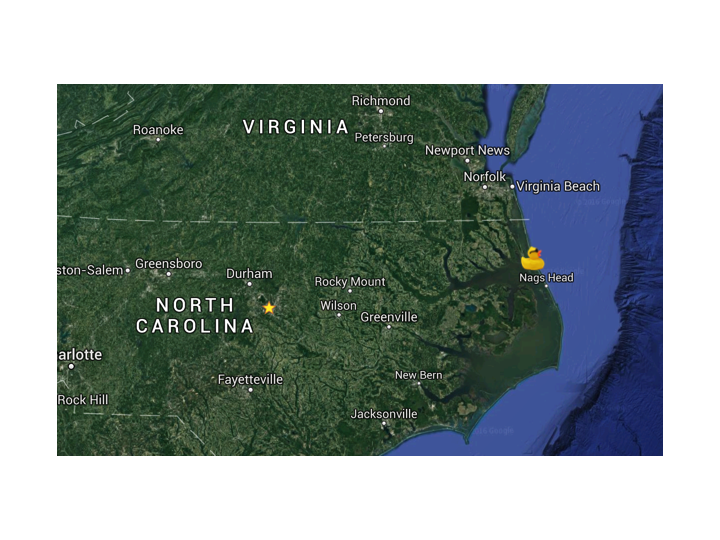
\includegraphics[width=1\linewidth]{img/map_ncsu_duck.png}
       		 \end{figure}
\end{frame}

%====================================================================================
% SLIDE 9
%====================================================================================
\begin{frame}
	\frametitle{Data includes $T$, $H$ at offshore boundary, 1D $k$}
		\begin{figure}[H]
			\centering
			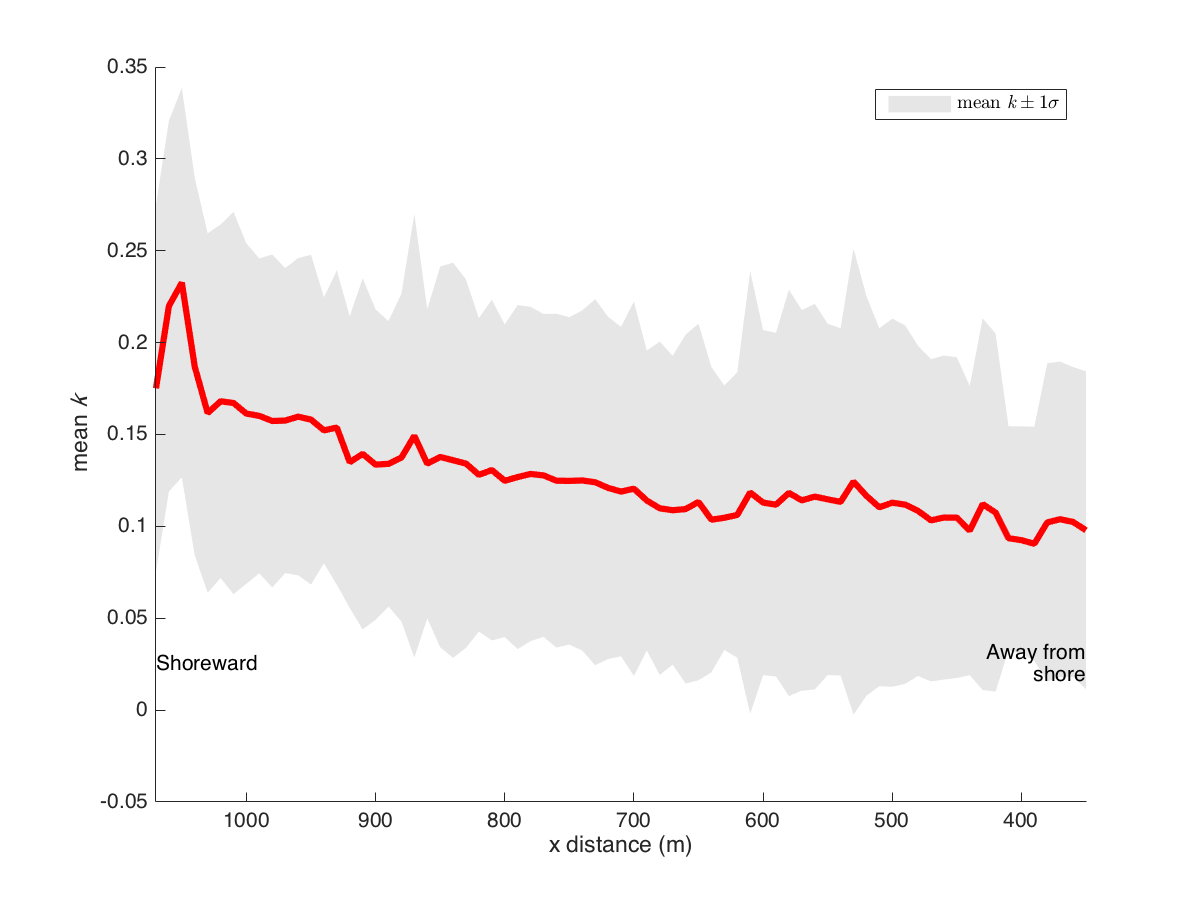
\includegraphics[width=1\linewidth]{img/k1Dmean_std.png}
		\end{figure}
\end{frame}


%====================================================================================
% SLIDE 10
%====================================================================================
\begin{frame}
	\frametitle{Known bathymetry is used for testing our results}
		\begin{columns}
			\column{0.5\textwidth}
				\begin{figure}[H]
	 				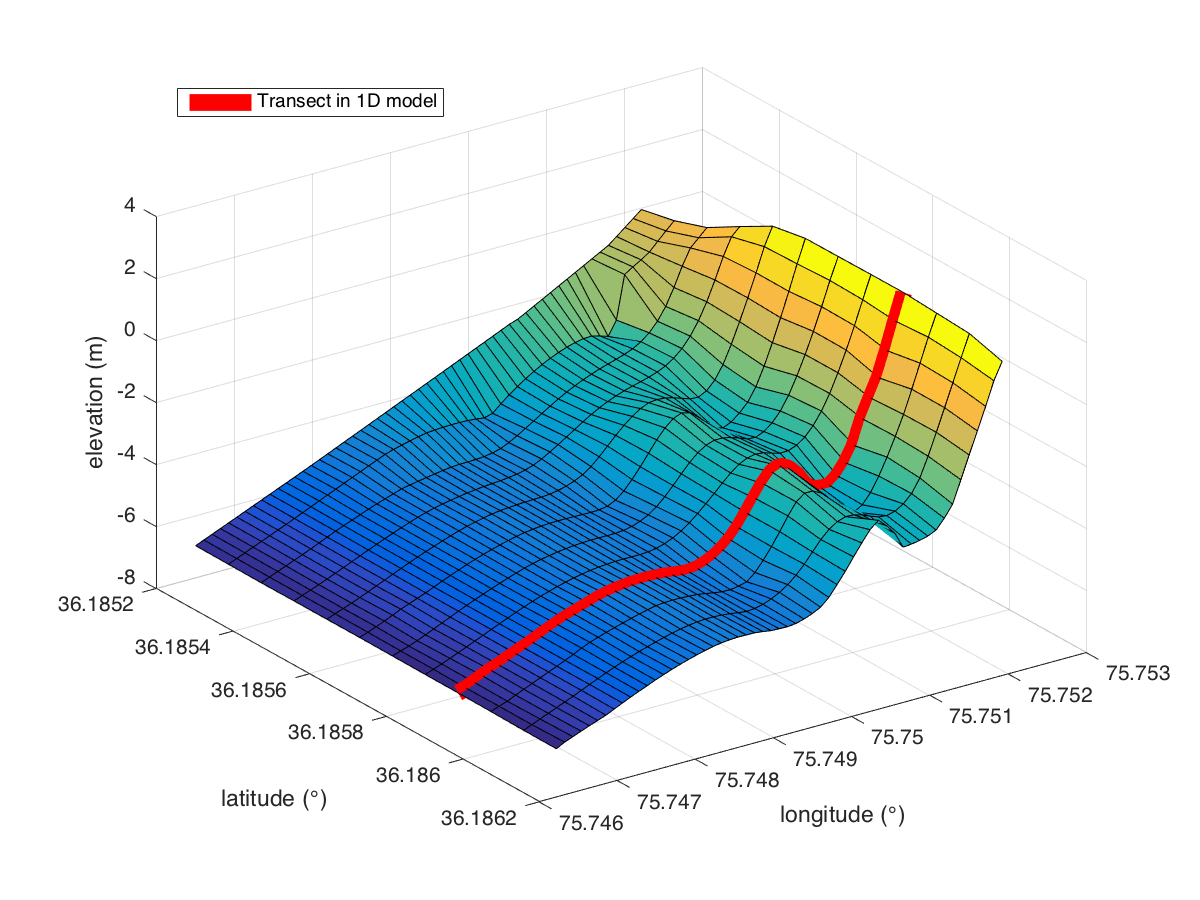
\includegraphics[width=1.2\linewidth]{img/trueBath2D.png}
	 			\end{figure}
			\column{0.5\textwidth}
				\begin{figure}[h]
					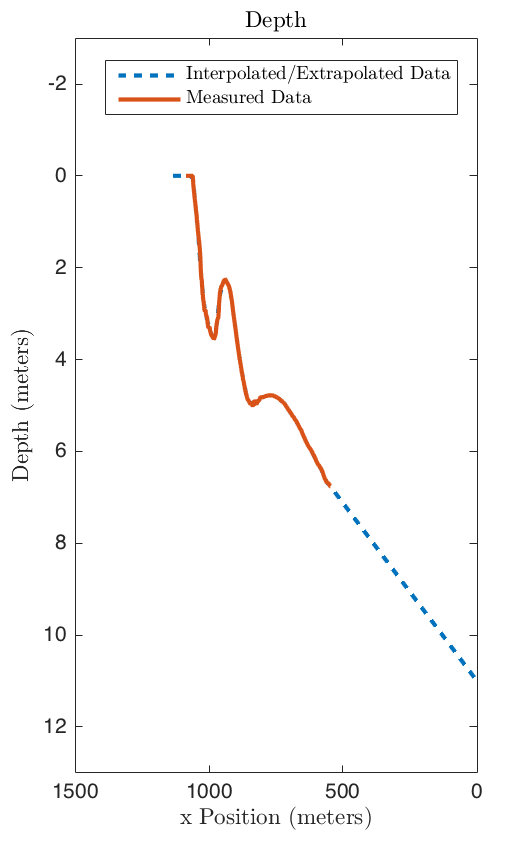
\includegraphics[width=.70\linewidth]{img/DepthChart.png}
				\end{figure}
			\end{columns}
\end{frame}

%==================================================================================
%==================================================================================
\section{Forward Model}
%==================================================================================
%==================================================================================

%==================================================================================
% SLIDE 11
%==================================================================================
\begin{frame}
 	\frametitle{Forward model computes $k$ assuming $h_{guess}$ \& BC}
		\begin{figure}[H]
	 		\centering
	 		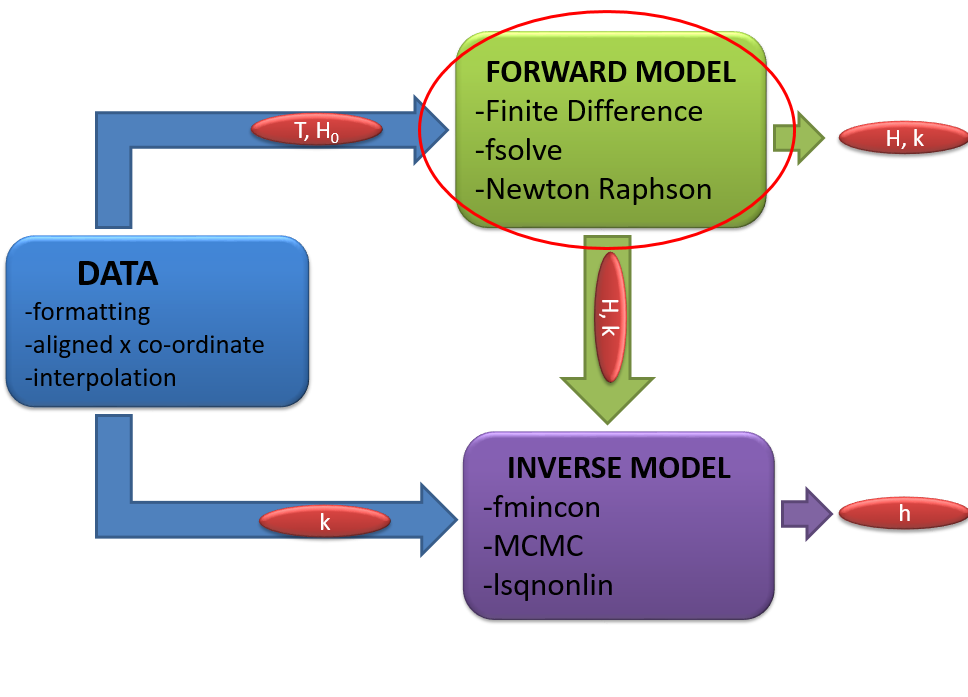
\includegraphics[width=1.0\linewidth]{img/FWD.png}
	 	\end{figure}
\end{frame}

%==================================================================================
%==================================================================================
\section{Inverse Methods}
%==================================================================================
%==================================================================================

%==================================================================================
% SLIDE 13
%==================================================================================
\begin{frame}
	\frametitle{1D wave physics is known for near-coastal regions}
		Assume linear wave theory:
		\begin{eqnarray*}
			\label{fp1}
			\left \{
				\begin{array}{lll}
					\frac{d}{dx}\left(EC_g\right)=-\delta,\\
					\\
					\sigma^2=gk\tanh(kh),
					\label{ode}
				\end{array}
			\right.
		\end{eqnarray*}
		\begin{equation*}
			\frac{d}{dx}\left( \frac{\lambda}{k}\left(1+\frac{2kh}{\sinh(2kh)}\right)H^2 \right)=-\delta
		\end{equation*}  
		\begin{flushleft}
			where,
		\end{flushleft}
		$${E: Wave \,Energy,\, C_{g}: Group \,celerity,}$$
		$${\quad c: Wave \,celerity,\, \sigma: Angular \,frequency,}$$
		$${\quad\quad\quad\quad g: Gravitational\,\, acceleration,k: Wave \,number}$$
\end{frame}

%==================================================================================
% SLIDE 14
%==================================================================================
\begin{frame}
 \frametitle{We invert for bathymetry given the surface data and physics}

\begin{figure}[flowchart]
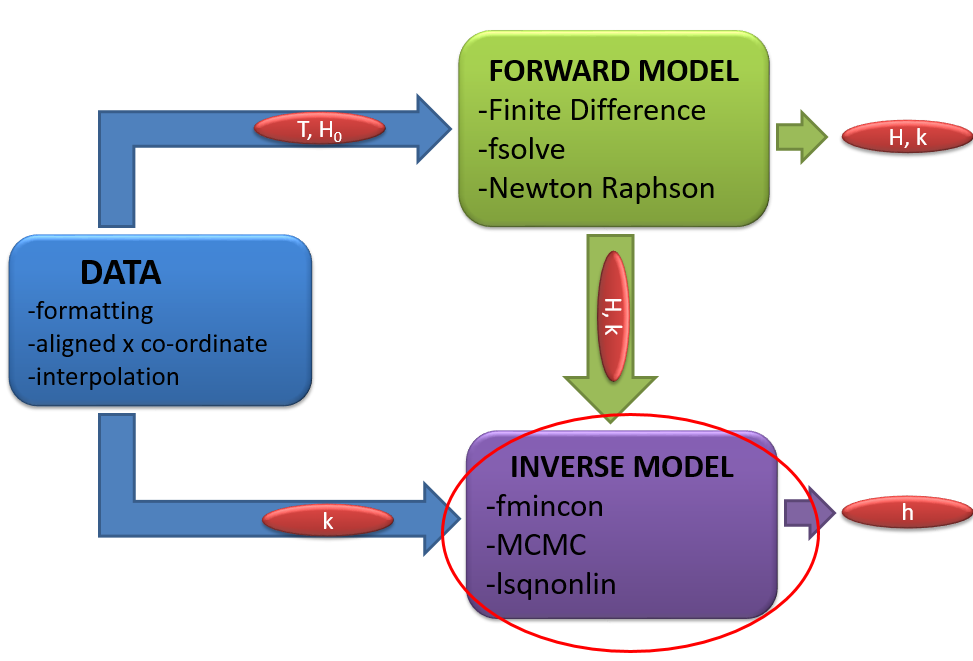
\includegraphics[width=1.0\linewidth]{img/INV.png}\hfill
%\captionsetup{labelformat=empty}
%\caption{Work flow of the project }
\end{figure}
%\end{columns}


\end{frame}
%==========================================================================================================================================
% SLIDE 8: We invert for bathymetry given the surface data and physics
%======================================================================================

\begin{frame}
 \frametitle{Inversion Methods}

\begin{itemize}
\item Nonlinear Least Squares
\item MCMC
\item fmincon
\end{itemize}

\end{frame}


%==========================================================================================================================================
% 
%======================================================================================
\subsection{Synthetic data}
\begin{frame}
 \frametitle{Synthetic Data}
\end{frame}

%==========================================================================================================================================
% 
%======================================================================================
\begin{frame}
 \frametitle{Synthetic Results plots for each}
\end{frame}

\subsection{Real data}
%==========================================================================================================================================
% 
%======================================================================================
\begin{frame}
 \frametitle{Real data for runs}
\end{frame}

%==========================================================================================================================================
% 
%======================================================================================
\begin{frame}
 \frametitle{Real Results plots for each}
\end{frame}

%==========================================================================================================================================
%SLIDE 16: Future directions fr IMSM 2017
\section{Discussion}
%==========================================================================================================================================
\begin{frame}
 \frametitle{Future Directions }
 \begin{itemize}
 \item Use of wave heights
 \item Regularization methods
 \item 2D problem
 \end{itemize}

\end{frame}
%=====================================================================================================
% Slide 17: THANK YOU
%==========================================================================================================
\begin{frame}
\frametitle{}
\hspace{2.5cm}
\begin{minipage}{50mm}   
                                                                                                                           
      \begin{alertblock}{}    
                                          
            \begin{center}
                                                                                                                                                                                  
                  \textbf{THANK YOU!}
                            
                                                                       
            \end{center}
      \end{alertblock}
\end{minipage}
\end{frame}

%==========================================================================================================================================
%==========================================================================================================================================
% SLIDE 9: We tried several inverse methods
%======================================================================================

%\begin{frame}
% \frametitle{We tried several inverse methods}
%\begin{itemize}
%\item Nonlinear least squares
%\item MCMC
%\item fmincon
%\end{itemize}
%\end{frame}
%==========================================================================================================================================

%SLIDE 14: fmincon
%==========================================================================================================================================
 \begin{frame}
\frametitle{Additive Gaussian Noise Model}

Gaussian noise $\boldsymbol{\epsilon}$ corrupted measurements $\mathbf{d}$ with variance $\nu$ is given by 
$$
\mathbf{d} = \mathbf{A} \mathbf{h}_t + \boldsymbol{\epsilon}.
$$

\begin{tabular}{l c l}
$\mathbf{d}$ &=& a vector of measurements,\\
$\mathbf{A}$ &=& a linear forward operator,\\
$\mathbf{h}_t$ &=& the true bathymetry. 
\end{tabular}

\end{frame}


%==========================================================================================================================================
%SLIDE 15: fmincon
%==========================================================================================================================================
 \begin{frame}
\frametitle{fmincon: Tikhonov Method}
\centering
Uses a regularized solution with prior information
$$
\mathbf{\hat{h}} = \underset{\mathbf{h} \in \mathbb{R}^n}{\arg \min} \|  \mathbf{A}\mathbf{h} -  \mathbf{d} \|_2^2  +  \alpha \| \mathbf{h} -  \mathbf{h}_p\|_2^2,
$$
\end{frame}

%==========================================================================================================================================
% SLIDE 11: Bayesian Markov Chain Monte Carlo (MCMC) Method
%======================================================================================

 \begin{frame}
\frametitle{Bayesian Markov Chain Monte Carlo (MCMC) Method}
The MCMC method creates a posterior distribution of depth profiles, given wave number by using the Bayes relationship

\begin{equation}\label{bayes}
P(h|%H,
k) \propto \Pi(h)L(h|%H,
k),
\end{equation} 
%\begin{itemize}
%\item $\Pi(h)$  prior distribution
%\item $L(h|%H,
%k)$ likelihood function
%\item $P(h|%H,
%k)$ posterior distribution
%\end{itemize}
\end{frame}

%==========================================================================================================================================
% SLIDE 13: MCMC Method: Metropolis Algorithm
%==========================================================================================================================================
\begin{frame}
 \frametitle{MCMC Method: Metropolis Algorithm}
\begin{itemize}
\item Prior and likelihood are combined to compute an initial posterior probability distribution of \textit{h}\\
\begin{equation}\label{post}
P(h|%H,
k) = log(\Pi(h)) + log(L(h|%H,
k))
\end{equation}
\item Uses a markov chain random walk to %propose and compare new \textit{h} profiles
arrive at a posterior distribution of \textit{h} profiles %which are expected to describe true bathymetry
\end{itemize}
\end{frame}
%==========================================================================================================================================
% SLIDE 10: Nonlinear least squares
%===================================================================================================================

 \begin{frame}
\frametitle{Nonlinear Least Squares: Trusted Region-Reflective Method}

\begin{equation}\label{LS}
\mathbf{\hat{h}}= \underset{\mathbf{h} \in \mathbb{R}^n}{\arg \min} \ \ f(\mathbf{h}) = \|  \mathbf{A}\mathbf{h} -  \mathbf{d} \|_2^2,
\end{equation}

\begin{figure}[H]
	 	\centering
	 	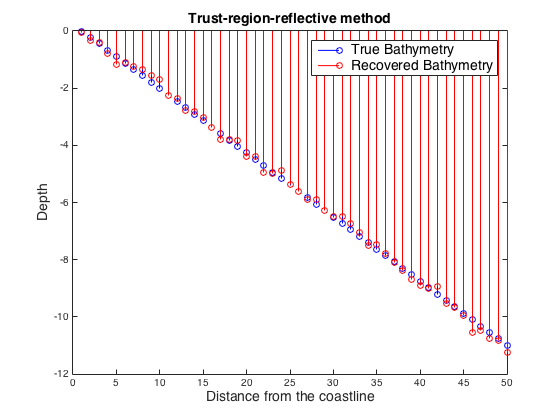
\includegraphics[width=.70\linewidth]{img/trust_region_linear.png}
	 	\end{figure}

\end{frame}

%==========================================================================================================================================
%SLIDE 1: Results
%==========================================================================================================================================
 \begin{frame}
\frametitle{Results}


\end{frame}


%==========================================================================================================================================




%===========================================================================================================================================
% SLIDE 12: MCMC Method: Log-Likelihood Function
%======================================================================================
\begin{frame}
 \frametitle{MCMC Method: Log-Likelihood Function}
 Loglikelihood function compares simulated and observed \textit{k} values

\begin{equation} \label{likely}
\log{L(h|%H,
k)}=log{e^{- \frac{\sum\limits_{i=1}^n({k}_{m,i}-k_{d,i})^2}{2\sigma_{d}^2}}}
\end{equation} 


\end{frame}
%==========================================================================================================================================


\end{document}

